\documentclass[14pt]{extbook}
\usepackage{multicol, enumerate, enumitem, hyperref, color, soul, setspace, parskip, fancyhdr} %General Packages
\usepackage{amssymb, amsthm, amsmath, latexsym, units, mathtools} %Math Packages
\everymath{\displaystyle} %All math in Display Style
% Packages with additional options
\usepackage[headsep=0.5cm,headheight=12pt, left=1 in,right= 1 in,top= 1 in,bottom= 1 in]{geometry}
\usepackage[usenames,dvipsnames]{xcolor}
\usepackage{dashrule}  % Package to use the command below to create lines between items
\newcommand{\litem}[1]{\item#1\hspace*{-1cm}\rule{\textwidth}{0.4pt}}
\pagestyle{fancy}
\lhead{Progress Quiz 4}
\chead{}
\rhead{Version A}
\lfoot{5346-5907}
\cfoot{}
\rfoot{Summer C 2021}
\begin{document}

\begin{enumerate}
\litem{
Solve the linear equation below. Then, choose the interval that contains the solution.\[ \frac{4x + 9}{3} - \frac{7x -6}{5} = \frac{-6x -6}{7} \]\begin{enumerate}[label=\Alph*.]
\item \( x \in [-6.7, -5.3] \)
\item \( x \in [-28.2, -25.3] \)
\item \( x \in [-3.2, -0.8] \)
\item \( x \in [-5.2, -2.7] \)
\item \( \text{There are no real solutions.} \)

\end{enumerate} }
\litem{
Solve the equation below. Then, choose the interval that contains the solution.\[ -12(-19x -11) = -18(-2x -5) \]\begin{enumerate}[label=\Alph*.]
\item \( x \in [-1.21, -0.9] \)
\item \( x \in [-0.86, -0.65] \)
\item \( x \in [0.48, 2.61] \)
\item \( x \in [-0.31, 0.24] \)
\item \( \text{There are no real solutions.} \)

\end{enumerate} }
\litem{
First, find the equation of the line containing the two points below. Then, write the equation in the form $ y=mx+b $ and choose the intervals that contain $m$ and $b$.\[ (7, -4) \text{ and } (-11, -10) \]\begin{enumerate}[label=\Alph*.]
\item \( m \in [-0.02, 1.47] \hspace*{3mm} b \in [4.33, 9.33] \)
\item \( m \in [-0.02, 1.47] \hspace*{3mm} b \in [-9.33, -2.33] \)
\item \( m \in [-0.79, 0.15] \hspace*{3mm} b \in [-17.67, -12.67] \)
\item \( m \in [-0.02, 1.47] \hspace*{3mm} b \in [-2, 3] \)
\item \( m \in [-0.02, 1.47] \hspace*{3mm} b \in [-13, -9] \)

\end{enumerate} }
\litem{
Write the equation of the line in the graph below in Standard Form $Ax+By=C$. Then, choose the intervals that contain $A, B, \text{ and } C$.
\begin{center}
    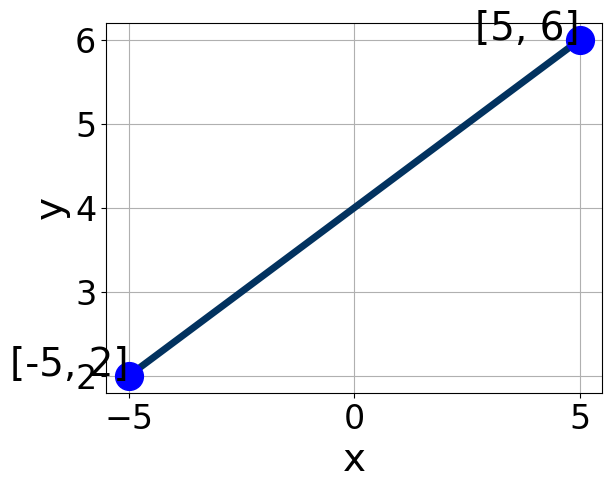
\includegraphics[width=0.5\textwidth]{../Figures/linearGraphToStandardCopyA.png}
\end{center}
\begin{enumerate}[label=\Alph*.]
\item \( A \in [-0.54, 0.83], \hspace{3mm} B \in [0.4, 1.3], \text{ and } \hspace{3mm} C \in [1, 5] \)
\item \( A \in [1.84, 2.92], \hspace{3mm} B \in [1.7, 6.9], \text{ and } \hspace{3mm} C \in [16, 28] \)
\item \( A \in [1.84, 2.92], \hspace{3mm} B \in [-5.6, -4.3], \text{ and } \hspace{3mm} C \in [-20, -14] \)
\item \( A \in [-0.54, 0.83], \hspace{3mm} B \in [-4.4, -0.7], \text{ and } \hspace{3mm} C \in [-8, -2] \)
\item \( A \in [-2.65, -1.44], \hspace{3mm} B \in [1.7, 6.9], \text{ and } \hspace{3mm} C \in [16, 28] \)

\end{enumerate} }
\litem{
Find the equation of the line described below. Write the linear equation in the form $ y=mx+b $ and choose the intervals that contain $m$ and $b$.\[ \text{Perpendicular to } 7 x + 9 y = 9 \text{ and passing through the point } (-7, -3). \]\begin{enumerate}[label=\Alph*.]
\item \( m \in [1.23, 2.14] \hspace*{3mm} b \in [5.2, 7.1] \)
\item \( m \in [1.23, 2.14] \hspace*{3mm} b \in [3.3, 4.4] \)
\item \( m \in [1.23, 2.14] \hspace*{3mm} b \in [-6.7, -2.7] \)
\item \( m \in [-1.31, -0.88] \hspace*{3mm} b \in [-15, -11.4] \)
\item \( m \in [0.52, 0.95] \hspace*{3mm} b \in [5.2, 7.1] \)

\end{enumerate} }
\litem{
Solve the equation below. Then, choose the interval that contains the solution.\[ -13(-16x -3) = -2(-6x -19) \]\begin{enumerate}[label=\Alph*.]
\item \( x \in [-0.01, 0.04] \)
\item \( x \in [-0.41, -0.38] \)
\item \( x \in [-0.35, -0.34] \)
\item \( x \in [0.39, 0.42] \)
\item \( \text{There are no real solutions.} \)

\end{enumerate} }
\litem{
Find the equation of the line described below. Write the linear equation in the form $ y=mx+b $ and choose the intervals that contain $m$ and $b$.\[ \text{Parallel to } 9 x + 7 y = 13 \text{ and passing through the point } (-6, -6). \]\begin{enumerate}[label=\Alph*.]
\item \( m \in [-1.36, -0.79] \hspace*{3mm} b \in [7.71, 16.71] \)
\item \( m \in [-1.36, -0.79] \hspace*{3mm} b \in [-14.71, -10.71] \)
\item \( m \in [-0.92, 0.06] \hspace*{3mm} b \in [-14.71, -10.71] \)
\item \( m \in [1.21, 1.32] \hspace*{3mm} b \in [1.71, 6.71] \)
\item \( m \in [-1.36, -0.79] \hspace*{3mm} b \in [-3, 1] \)

\end{enumerate} }
\litem{
Write the equation of the line in the graph below in Standard Form $Ax+By=C$. Then, choose the intervals that contain $A, B, \text{ and } C$.
\begin{center}
    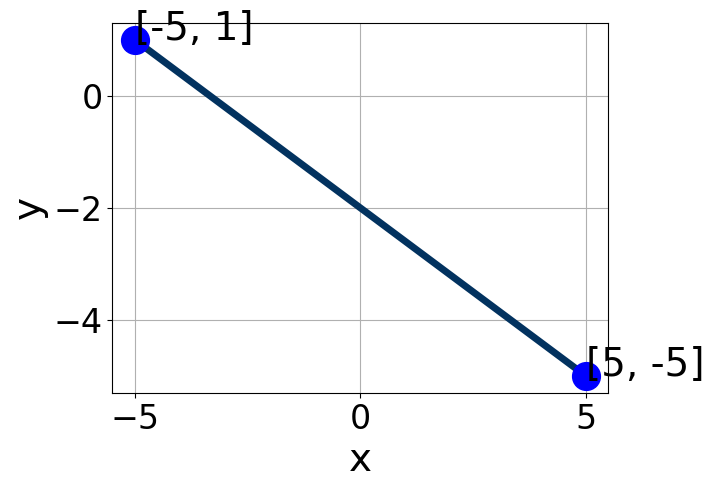
\includegraphics[width=0.5\textwidth]{../Figures/linearGraphToStandardA.png}
\end{center}
\begin{enumerate}[label=\Alph*.]
\item \( A \in [-2.4, 2.6], \hspace{3mm} B \in [-0.4, 1.8], \text{ and } \hspace{3mm} C \in [-2, 0] \)
\item \( A \in [1, 6], \hspace{3mm} B \in [2.9, 5.2], \text{ and } \hspace{3mm} C \in [-15, -7] \)
\item \( A \in [-8, -2], \hspace{3mm} B \in [-5.8, -4.3], \text{ and } \hspace{3mm} C \in [10, 12] \)
\item \( A \in [-2.4, 2.6], \hspace{3mm} B \in [-4, -0.7], \text{ and } \hspace{3mm} C \in [2, 3] \)
\item \( A \in [1, 6], \hspace{3mm} B \in [-5.8, -4.3], \text{ and } \hspace{3mm} C \in [10, 12] \)

\end{enumerate} }
\litem{
Solve the linear equation below. Then, choose the interval that contains the solution.\[ \frac{-4x -7}{8} - \frac{4x + 4}{3} = \frac{-4x + 9}{4} \]\begin{enumerate}[label=\Alph*.]
\item \( x \in [-25.1, -22.8] \)
\item \( x \in [-3.9, -1.2] \)
\item \( x \in [-1.5, 0.2] \)
\item \( x \in [-6.2, -4.7] \)
\item \( \text{There are no real solutions.} \)

\end{enumerate} }
\litem{
First, find the equation of the line containing the two points below. Then, write the equation in the form $ y=mx+b $ and choose the intervals that contain $m$ and $b$.\[ (8, -5) \text{ and } (-7, -6) \]\begin{enumerate}[label=\Alph*.]
\item \( m \in [0.05, 0.24] \hspace*{3mm} b \in [-5.7, -3.4] \)
\item \( m \in [0.05, 0.24] \hspace*{3mm} b \in [-0.7, 2.9] \)
\item \( m \in [-0.22, 0.02] \hspace*{3mm} b \in [-7.4, -6.1] \)
\item \( m \in [0.05, 0.24] \hspace*{3mm} b \in [3.5, 7.5] \)
\item \( m \in [0.05, 0.24] \hspace*{3mm} b \in [-14.3, -12.7] \)

\end{enumerate} }
\end{enumerate}

\end{document}